\documentclass[12pt]{ctexart}
\usepackage{amssymb,amsmath,makecell}
\usepackage{hyperref}
\usepackage{booktabs}
\usepackage[nofonts]{ctexcap}
\usepackage{setspace}
\usepackage{graphicx}
\usepackage{fix-cm}
\usepackage{enumerate}
\usepackage{float}
\usepackage{graphicx}
\usepackage{fancybox}
\usepackage{longtable}
\usepackage{multirow}
\usepackage{minted}
\usepackage{minipage-marginpar}
\usepackage{pdfpages}
\usepackage{paralist}
\usepackage[linesnumbered,ruled,vlined]{algorithm2e}
\usepackage[normalem]{ulem}
\useunder{\uline}{\ul}{}
\usepackage{tikz}
\usetikzlibrary{automata, positioning, arrows.meta, arrows}

\usepackage[bjydu]{cnlogo}
\definecolor{bjydu}{RGB}{0,51,153}

\newmintinline{cpp}{breaklines,breakanywhere}
\newminted{cpp}{breakanywhere,breaklines,linenos,frame=single}

\newcommand{\bigsize}{\fontsize{25pt}{20pt}\selectfont}
% \setCJKmainfont[BoldFont=STFangsong]{STFangsong}
% Page length commands go here in the preamble
\setlength{\oddsidemargin}{-0.25in} % Left margin of 1 in + 0 in = 1 in
\setlength{\textwidth}{7in}   % Right margin of 8.5 in - 1 in - 6.5 in = 1 in
\setlength{\topmargin}{-.75in}  % Top margin of 2 in -0.75 in = 1 in
\setlength{\textheight}{9.2in}  % Lower margin of 11 in - 9 in - 1 in = 1 in

\newtheorem{theorem}{Theorem}
\newtheorem{definition}{Definition}

\renewcommand{\baselinestretch}{1.5} % 1.5 denotes double spacing. Changing it will change the spacing

\hypersetup{colorlinks=true,linkcolor=black,filecolor=magenta,urlcolor=cyan}
\setlength{\parindent}{0in}

\begin{document}
% \CTEXsetup[format={\Large\bfseries}]{section}
% \CTEXsetup[number={\chinese{section}}]{section}
\begin{titlepage}
    \center
    
\includegraphics[width=3.5in]{images/buptname.eps}

    \begin{spacing}{5}
        {\bigsize \textbf{设计报告}}
    \end{spacing}

    % \includegraphics[width=2.3in]{images/buptseal.eps}
    \bjydulogo[bjydu][1.8]

    \begin{spacing}{1}
        \vspace{1.5cm}
        \Large \begin{tabular}{@{}l@{}} % @{}用于消除列前后的空格
            课程名称: 编译原理与技术                \\
            实验名称: 语法分析               \\
            学\qquad 院: 计算机学院               \\
            班\qquad 级: 2022211312          \\
            学\qquad 号: 2022211404          \\
            姓\qquad 名: 唐梓楠
        \end{tabular}
        \vspace{2.5cm}
    \end{spacing}

    \title{语法分析设计报告}
    \author{唐梓楠}

    {\small\em \today }
\end{titlepage}


\newpage

\tableofcontents

\newpage
\section{什么是 lex/flex?}

\subsection{程序设计说明}

使用 lex/flex 实现对以小写字母 ab 结尾的字符串 (只包含大小写字母) 的识别,如 Helloab 和 Goab.

\subsection{测试报告}

该题较为简单, 使用正则表达式表达以 ab 结尾的纯字母字符串即可. 通过参考 \href{https://westes.github.io/flex/manual/}{flex 手册的第七章}, 可以得到如 \autoref{fig:pattern} 所示的正则表达式规则. \begin{figure}[htbp]
    \centering
    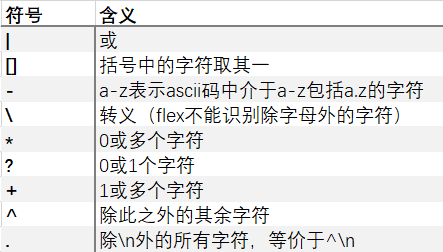
\includegraphics[width=0.5\textwidth]{images/pattern.png}
    \caption{flex patterns}
    \label{fig:pattern}
\end{figure}

根据规则, 可以构造出表达式即: \begin{cppcode}
 /* begin */
 [a-zA-Z]*ab    {printf("%s: Hit!\n", yytext);}
 /* end */
\end{cppcode}

需要注意的是, 使用 flex 时正则表达式前面不能有空格或缩进, 否则会报错.

\section{用 flex 生成 PL 语言的词法分析器}

\subsection{程序设计说明}

利用 flex 工具生成 PL 语言的词法分析器, 要求输入一个 PL 语言源程序文件 \texttt{demo.pl},输出一个文件 \texttt{tokens.txt}, 该文件包括每一个单词及其种别枚举值, 每行一个单词.

此外还有一个类别 \texttt{ERROR}, 包括不是出现在字符串中的非法字符,  当词法分析器读到非法字符时, 应该输出 \texttt{ERROR} 作为种别值.

\subsubsection{具体实现}

PL 语言单词的符号及其种别值如 \autoref{fig:PL_words} 所示: \begin{figure}[htbp]
    \centering
    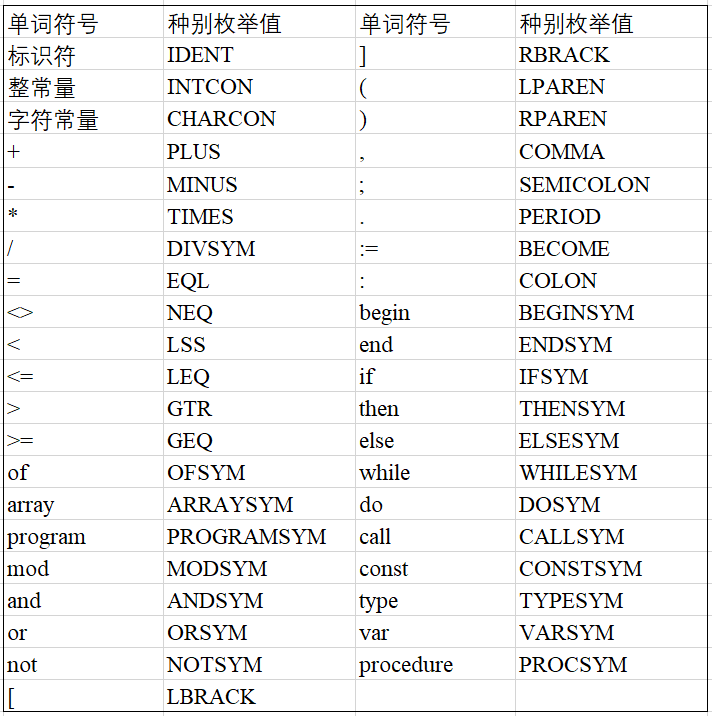
\includegraphics[width=0.5\textwidth]{images/PL_words.png}
    \caption{PL 语言单词符号及其种别值}
    \label{fig:PL_words}
\end{figure}

可以构建 PL 单词的状态图如 \autoref{fig:PL_state} 所示. \begin{figure}[htbp]
    \centering
    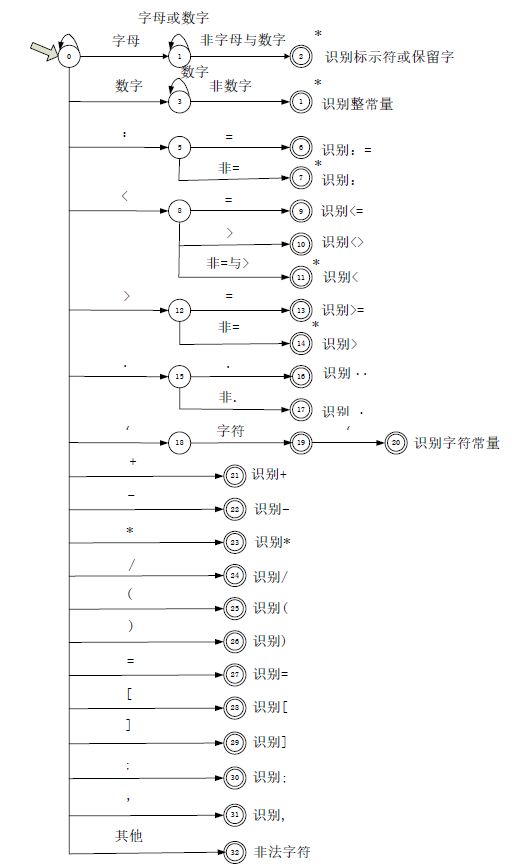
\includegraphics[width=0.8\textwidth]{images/PL_state.png}
    \caption{PL 单词状态图}
    \label{fig:PL_state}
\end{figure}

\subsection{测试报告}

大部分状态按照状态图, 根据 flex 语言的正则表达式模式就可以轻松完成.

需要注意的是优先级顺序, 应该将优先级高的对应正则表达式子放在前面, 低的放在后面, 最后处理 \texttt{ERROR}.

比较困难的是对于字符常量 \texttt{CHARCON} 的识别.

\subsubsection{识别 \texttt{CHARCON}}

\textbf{输入}: \verb|'shuebqbdhh_fye788893\da"'|

\textbf{运行结果}: \texttt{CHARCON}

\textbf{分析说明}: 首先用 \verb|\'| 匹配单引号 \verb|'|,即字符常量的开头和结尾。重点在于内部字符常量的内容识别逻辑. \begin{itemize}
    \item \verb|[^'\\]| 表明这是一个字符类,用来匹配任何不是单引号 \verb|'| 和反斜杠 \verb|\| 的字符。也就是说,这里匹配除了单引号和反斜杠以外的普通字符。
    \item \verb|\\.| 表示匹配反斜杠 \verb|\| 后跟任意字符的情况。由于字符常量可能包括转义字符,如 \verb|\'| 或 \verb|\\|,因此这一部分用于处理这些转义字符。与前者用 \texttt{|} 连接.
    \item 用 \verb|*| 表示前面部分可以匹配零次或多次,即允许字符常量的内容部分可以包含任意长度的符合规则的字符。
\end{itemize}

设计出的正则表达式为: \begin{cppcode}
CHARCON         \'([^'\\]|\\.)*\'
\end{cppcode}

该正则表达式可以匹配由单引号包围的字符常量, 内容部分可以是除单引号和反斜杠外的任意字符, 或者是反斜杠后跟的转义字符 (如 \verb|\'|, \verb|\\| 等). 整个表达式确保字符常量以单引号开头和结尾, 并且允许其中包含合法的转义序列.

\section{词法分析程序的设计与实现(C/C++)}

\subsection{程序设计说明}

设计并实现一个 C 语言的词法分析程序。

要求: \begin{enumerate}
    \item 识别单词符号并以记号形式输出,并标出该单词符号所在行数。应考虑的单词符号见输出格式;
    \item 能够识别并跳过注释;
    \item 能够检查到错误的词法;
    \item 能够统计行数、各个单词符号的类别数, 以及词法错误数.
\end{enumerate}

本题的状态转化图与书上类似, 因此我以书上的状态转化实现为基础, 如 \autoref{fig:state} 所示, 进行拓展完善,实现了自动机的状态转化, 并实现了与教材一致的配对缓冲区. 设计思路也保持与教材实现一致. 具体可参考代码. \begin{figure}[htbp]
    \centering
    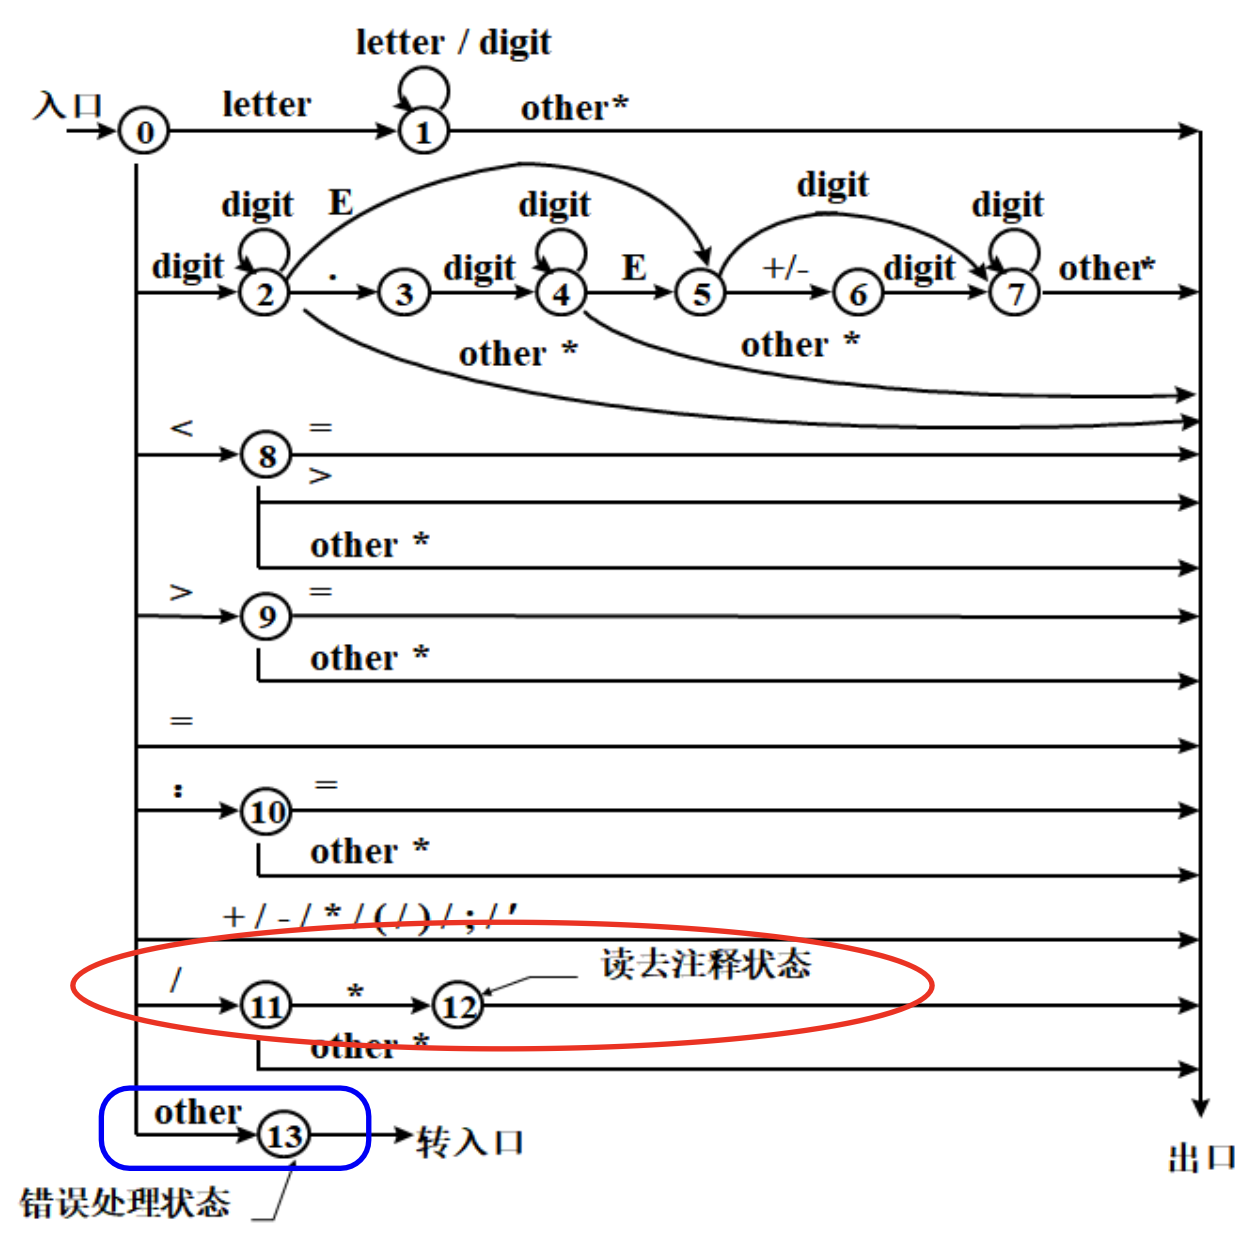
\includegraphics[width=0.5\textwidth]{images/state.png}
    \caption{基本状态图}
    \label{fig:state}
\end{figure}

\subsubsection{配对缓冲区实现}
缓冲器分为大小相同的两半, 每半包含 \texttt{N} 个字符, 且每半区带有结束标记, 减少比较次数.
\begin{cppcode}
void get_char()
{
    if (buffer[forwardptr] == '\0') {
        if (forwardptr == HALF_SIZE - 1) {
            file.read(buffer + HALF_SIZE, HALF_SIZE - 1);
            add_eof(HALF_SIZE);
            ++forwardptr;
        } else if (forwardptr == BUFFER_SIZE - 1) {
            file.read(buffer, HALF_SIZE - 1);
            add_eof(0);
            forwardptr = 0;
        }

        if (buffer[forwardptr] == '\0') {
            file.close();
            cout << line_cnt << '\n';
            cout << keywords_cnt << ' ' << identifiers_cnt << ' ' << operators_cnt << ' ' << delimiters_cnt << ' ' << charcons_cnt << ' ' << strings_cnt << ' ' << numbers_cnt << '\n';
            cout << errors_cnt;
            exit(0);
        }
    }
    C = buffer[forwardptr];
    ++forwardptr;
}
\end{cppcode}

\subsubsection{常量表数据结构}

在存储如关键字和保留字常量表时, 为了实现高效率, 我们使用了 STL 中的 \texttt{unordered\_set} 来存储, 其内部采用哈希表实现, 能够在 $O(1)$ 的时间复杂度内完成查找操作, 相较于普通的 \texttt{set} 有性能上的优势.   

\subsubsection{完整转换图}

根据 C11 语言 (参考草案: \href{https://open-std.org/JTC1/SC22/WG14/www/docs/n1570.pdf}{ISO/IEC 9899:201x}) 标准, 我们可以构造出如下的状态转移图:

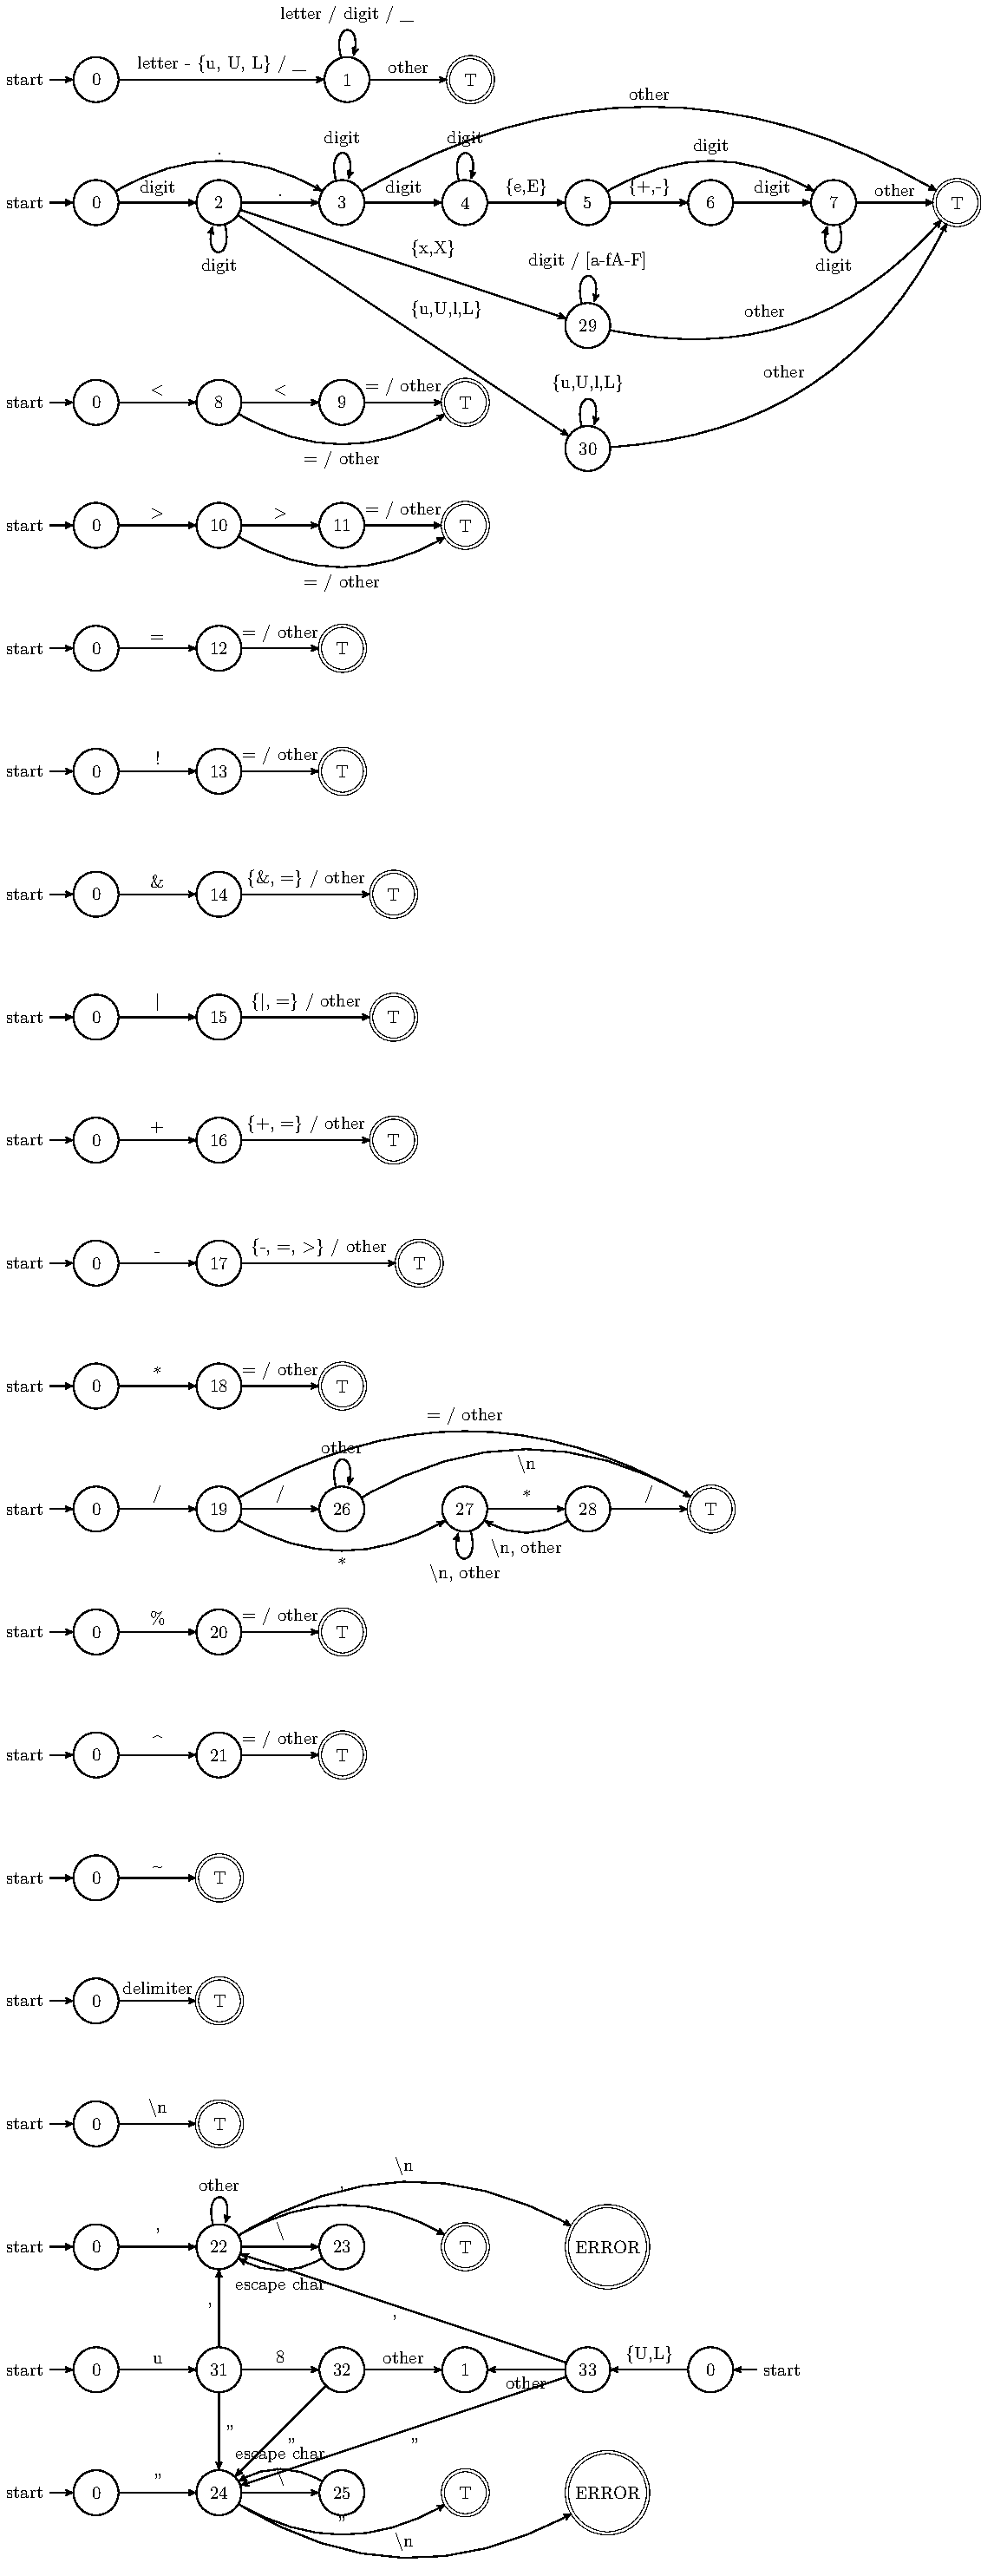
\includepdf[pages=-]{figure.pdf}

根据状态转移图, 我们可以很轻松的用 \texttt{switch case} 语句实现有限状态自动机.

\subsection{测试报告}

基础的前20个测试集较为简单, 只需对照状态转化图实现即可, 我们主要分析扩展要求中的 21-25 测试集.

\subsubsection{对合法的不带后缀的八进制数与十六进制数的识别}

\textbf{输入}: \verb|0x1ABCD2F|

\textbf{输出}: \verb|<NUMBER,0X3abcde2>|

\textbf{分析说明}: 由于八进制数与十六进制数的特殊性, 我们需要对其进行特殊处理. 八进制数以 \verb|0| 开头, 十六进制数以 \verb|0x| 或 \verb|0X| 开头. 识别到开头后, 循环识别数字即可, 需要注意的是, 十六进制数字可能包含 \verb|A-F| 或 \verb|a-f|.

\subsubsection{对合法的带后缀的十进制数的识别}

\textbf{输入}: \verb|107LLu|

\textbf{输出}: \verb|<NUMBER,107LLu>|

\textbf{分析说明}: 带后缀的十进制数以 \verb|L| 或 \verb|l| 结尾, 也可以以 \verb|U| 或 \verb|u| 结尾, 也可以同时出现. 识别到数字后, 循环识别后缀即可.

\subsubsection{考虑完整的浮点型常量的识别}

\textbf{输入}: \verb|.001e2f|

\textbf{输出}: \verb|<NUMBER,.001e2f>|

\textbf{分析说明}: 相较于一般的浮点数, 这里完整的浮点数识别还包括后缀, 用同样的方法添加后缀识别即可. 此外, 还需要注意可以省略最开头的 0, 因此识别到 \. 时, 需要增加对数字的跳转.

\subsubsection{带前缀的字符串常量的识别}

\textbf{输入}: \verb|u8"ABC"|

\textbf{输出}: \verb|<STRING,u8"ABC">|

\textbf{分析说明}: 带前缀的字符串常量以 \verb|u8|, \verb|u|, \verb|U|, \verb|L|开头, 识别到前缀后, 识别到 \verb|"| 后, 循环识别字符串即可. 因此不能将上述几个字符作为普通的 \texttt{letter} 处理, 应该进行额外的判断.

\subsubsection{完整的字符常量的识别}

\textbf{输入}: \verb|'abc'|

\textbf{输出}: \verb|<CHARCON,'abc'>|

\textbf{分析说明}: 这里定义的字符常量比较奇怪, 可以包括任意长度的字符, 和字符串区别不大, 原来在这里纠结了很久为什么可以这么表达, 查阅了 C 语言的相关资料也并没有相关的定义, 因此这里只能最后只能按照题目要求进行实现. 最后字符常量 \verb|CHARCON| 和字符串 \verb|STRING| 的差异不大了, 区别体现在对换行的报错.

\subsubsection{字符串}

\textbf{输入}: \begin{cppcode}
    /*
    */
\end{cppcode}

\textbf{输出}: 无

\textbf{分析说明}: 用 \texttt{/*} 开头, 且用 \texttt{*/} 结尾的注释是支持换行的, 但是测试集中并没有涉及到换行的情况.

\section{线上测试例通过情况截图}

\begin{figure}[htbp]
    \centering
    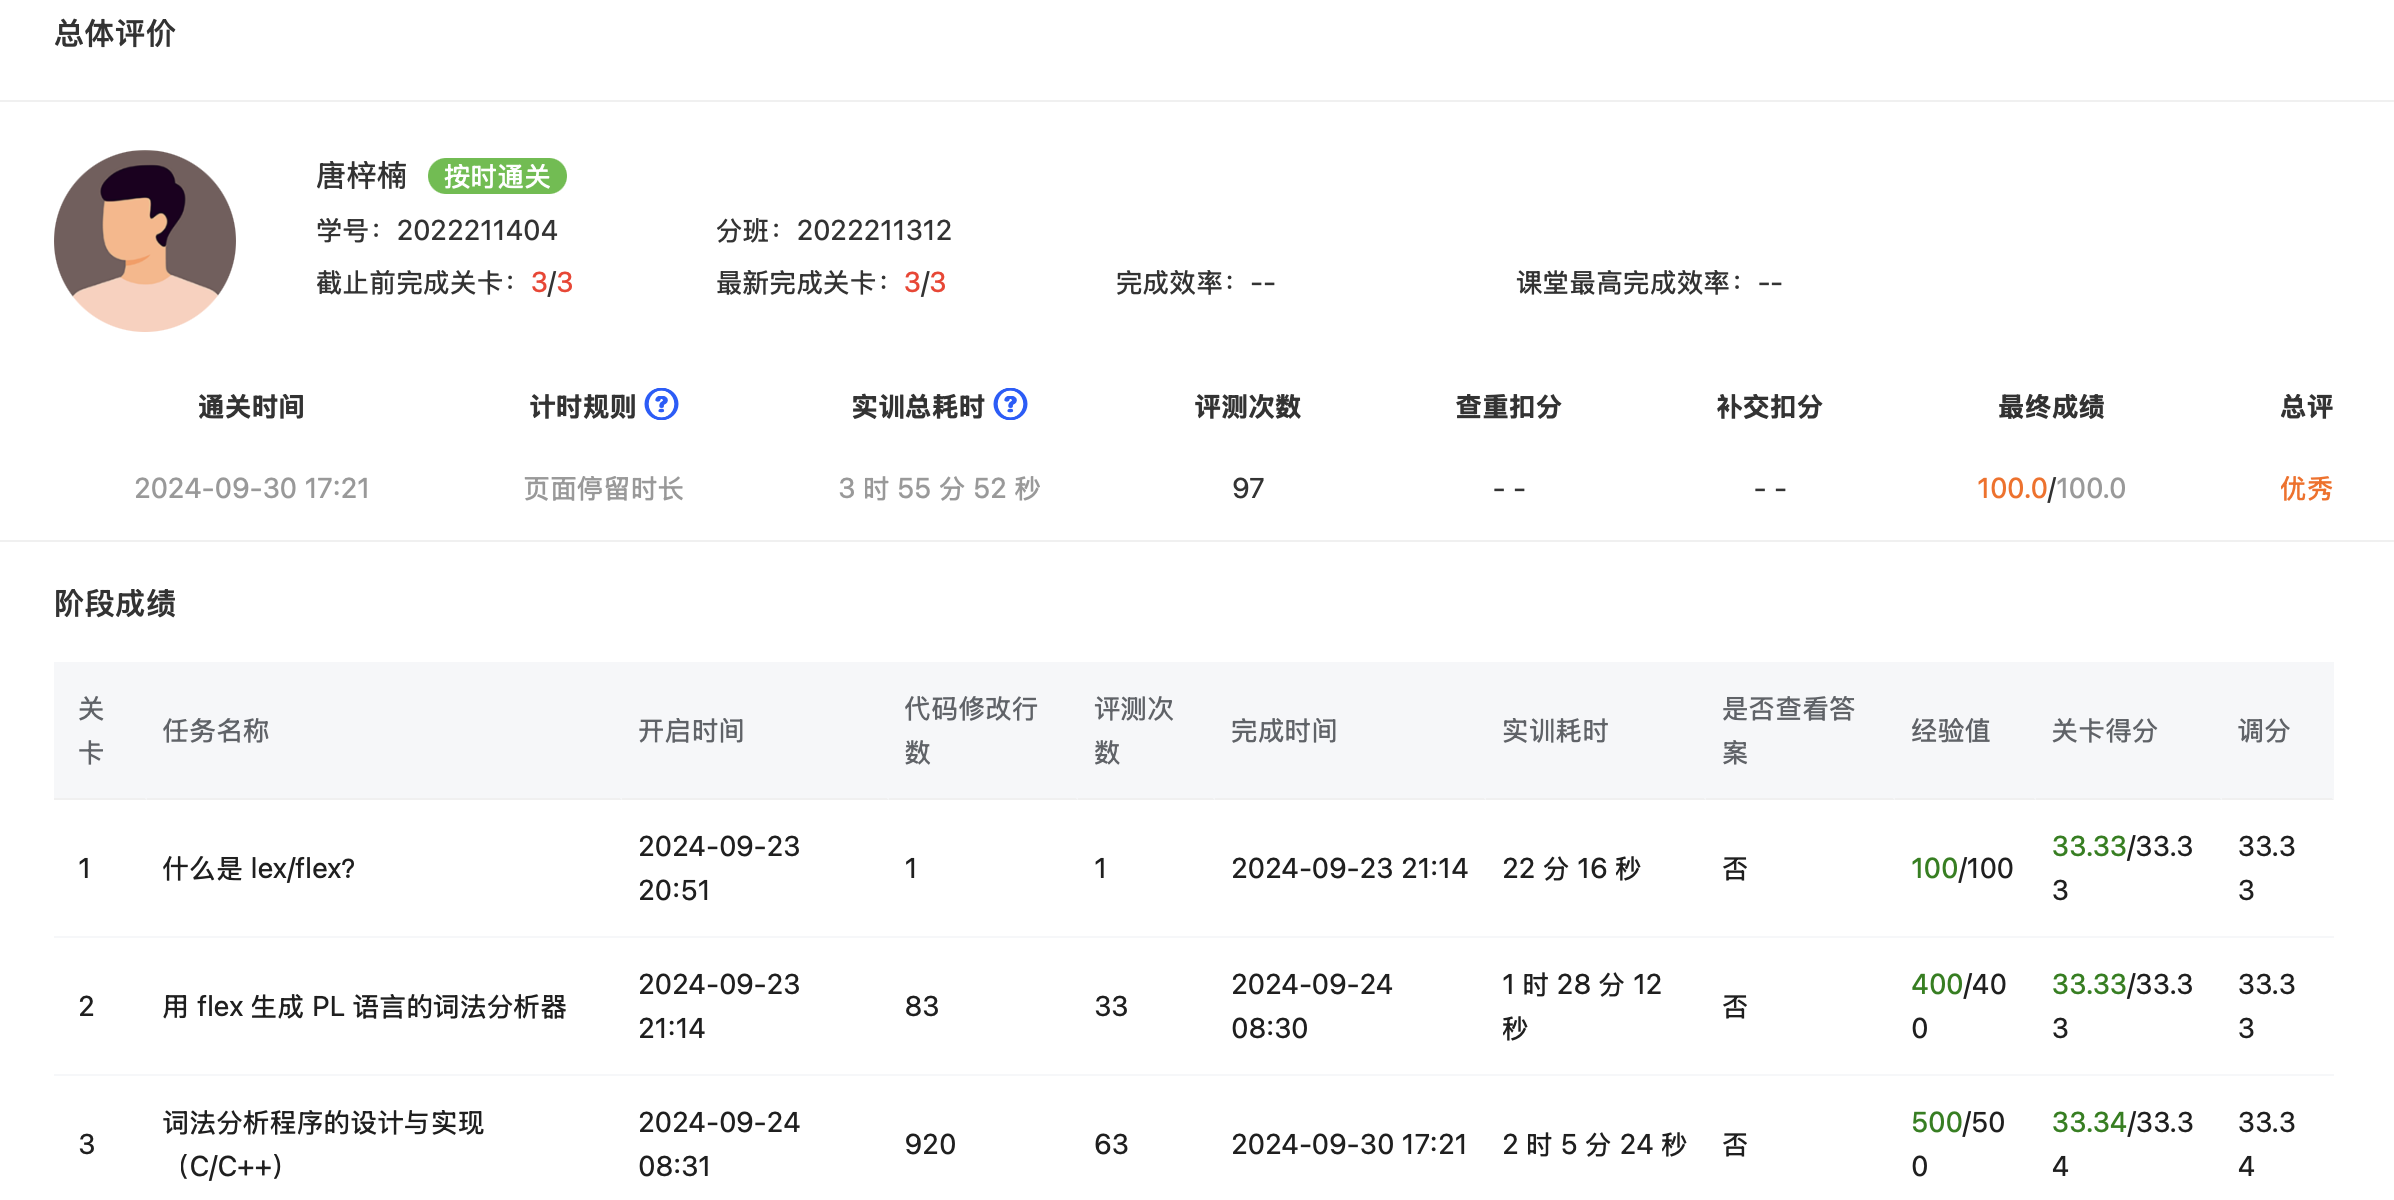
\includegraphics[width=0.8\textwidth]{images/score.png}
    \caption{全部通过 (包括附加内容)}
\end{figure}
\end{document}
